\section{Metric choice: Datacenter placements in renewable power grid}
\label{sec:quantify}
%PLEASE INCLUDE THIS/APPROPRIATELY EDITED FORM OF THIS TEXT IN INTRODUCTION%%%%
%Today many datacenters are being powered by renewable energy source like wind and solar. There are two choices of locating the datacenters i) near the wind or solar farm, what we refer to as co-location in the paper or ii) away from the renewable energy source (power is transmitted over long distance transmission lines). This paper answers the questions i) how do we decide which of the two is better and ii) how do we plan the datacenter location if we have multiple choices. In order to decide which one of these choices are better we need to define a comprehensive metric. In this paper we will first define these metrics and justify by considering a realistic scenario of placing datacenter in the New England system. Later, we provide a planning methodology that can be used to determine the datacenter location in any electric grid with wind or solar power. Finally, we propose an optimization algorithm that can be used to determine the best datacenter location under a given set of constraints.
%%%%%%%
Planning optimal datacenter location, requires comprehensive metric definition. Most of the studies carried out so far neglect the impact of renewable powered datacenters on the transmission grid. When the penetration of renewable powered datacenters was small, the impact of these on the transmission grid was insignificant. However, with several large datacenter companies opting for renewable energy source it becomes imperative to study their impact on the transmission grid.


\subsection{Simulation study}
In order to study the impact of datacenter location in a renewable power grid we consider the New England ISO transmission network. We choose this system due to the following reasons:
\begin{itemize}
\item{Wind power expansion in New England: The system studies carried by the New England ISO state that in this region there is a potential of integrating up to 12 Giga-Watts of wind power. Given this enormous interest to install new wind farms, this region may have a great potential in future to accommodate datacenters powered by wind farms.}
\item{Transmission network upgrades: A study carried out by the New England ISO showed that they could potentially integrate wind resources to meet up to 24\% of the region's total annual electric energy needs in 2020 if the system includes transmission
upgrades. If these transmission upgrades can be limited then the development of new wind farms becomes more economical.}
\item{Positive impacts of wind power in New England ISO: Introducing large amounts of low-marginal-cost wind generation tended to depress the spot price and reduce the price differential for bulk power between day and night. Also the study results demonstrated that there was only a relatively small increase in the use of existing pumped-storage hydro power for large wind penetrations, largely because the flexible natural-gas-fired generation fleet provided most of the system balancing.}
\end{itemize}
We will show in our study, that within the New England ISO, the wind power penetration can be increased much more cost effectively by strategically locating the datacenter. Intuitively, it may appear that co-locating datacenter loads and wind farms would solve the problem of building new transmission lines, limit the voltage variation and also minimize losses. However, our study shows that this is not indeed true and co-locating wind farm and datacenter may not be the optimal solution always.
\subsubsection{Model of the New England renewable power datacenter}
Before we carry out the case studies, we will describe the approximations we made and the models we used for each sub-system we considered in our study.
\begin{itemize}
\item{New England transmission system model: \\
For our study we considered a widely used  \cite{bills1970line} model of the New England transmission network. A single line diagram of this test system is shown in Figure~\ref{fig:newengland}. As shown in the figure, the model lumps all the generators, loads and transmission lines in the New England ISO region to 10 generators, 19 loads and 46 lines and transformers. The 10 generator buses are numbered from 30-39 in Figure~\ref{fig:newengland}. Specifically, bus 39 represents the aggregation of a large number of generators interconnected to rest of US/Canada.

%%%
\begin{figure}[ht]
\centering
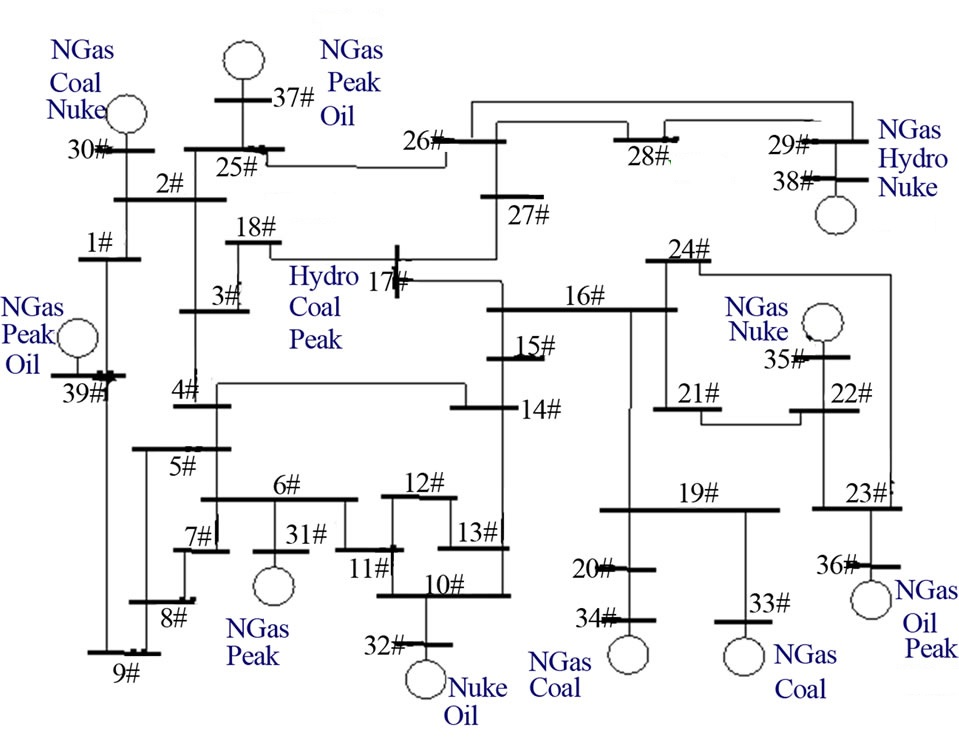
\includegraphics[width=1\columnwidth]{img/newEngland.jpg}
\caption{New England 39 bus test system}
\label{fig:newengland}
\end{figure}
%%%
}

\item{Datacenter model: \\
Based on the geographical mapping we aggregate all the datacenters in the New England ISO region into six datacenters, each datacenter for one state. In order to estimate the size of an "aggregated" datacenter in a certain state, we sue the follow equation:

\begin{equation}
L_i=\frac{n_i*9.8GW}{1278}
\end{equation}

\noindent where $L_i$ is the aggregated load of the $i$th state, $n_i$ is the number of datacenters reported in that state,  9.8GW is the upper bound of total electricity used by US datacenters in 2010, according to the report \cite{Koomey2011}, and 1278 is the number of datacenters in US collected and reported in \cite{DCmap}. However, according to \cite{Koomey2011}, for the summarized load of datacenters, there is an increase of 56\% from 2005-2010. Hence, we are assuming the increasing percentage from 2010-2014 is 56\%*0.8=45\%, and after adjustment we are using $L'_i=1.45L_i$ as the datacenter load for the target grid system.

The state wise aggregated datacenters are mapped to different buses according to their geographical locations, as seen from Table~\ref{tab:dc_setting}. Note that the load size given in the table represents the total load of datacenters in the entire state.

\begin{table}[ht]
\begin{center}
\caption{Background datacenter load and location settings}
\begin{tabular}{|l|l|p{30pt}|p{30pt}|p{30pt}|}
\hline
DC No. & State & Number of DCs & Estimated size(MW) & Mapped Bus No.\\
\hline
DC1 & Connecticut & 12 &133.43 & 6\\
DC2 & Maine & 3 &33.36 & 29 \\
DC3 & Vermont & 4 &44.48 & 25 \\
DC4 & Rhode Island & 3 &33.36 & 20\\
DC5 & New Hampshire & 4& 44.48 & 16\\
DC6 & Massachusetts & 27& 300.21 & 4 \\
\hline

\end{tabular}
   \vspace{.05in}
\label{tab:dc_setting}
\end{center}
\end{table}
}

\item{Wind farm model: \\
The wind farms connected to bus 18, 28, 36, 37 and 38 (Figure~\ref{fig:newengland}) are lumped models of several wind farms within a geographical region. The locations and capacity settings of the five wind farms are presented in Table~\ref{tab:wf_setting}. We assume that each farm can be represented by `$n$' identical wind turbines, where $n$= total farm rated capacity/individual wind turbine rating. This approximation does not change any of our results because we are interested in studying the global impact of wind farm powered datacenters on the electric grid. Also, since most of the wind turbines in this region are the GE 1.5MW machines, we consider the GE machine wind speed versus power characteristics \cite{lei2006modeling}. The wind speed versus turbine output characteristics is commonly referred to as the power curve (Figure~\ref{fig:windcurve}). From Figure~\ref{fig:windcurve} we can see that the cut-in wind speed, i.e., the wind speed at which the turbine starts producing power, is 5m/s and the cut-off wind speed is 25m/s, beyond this the turbine will be shut down for safety reasons. The wind turbine produces rated output (1.5MW) between wind speeds of 13-25m/s.
%%%
\begin{figure}[ht]
\centering
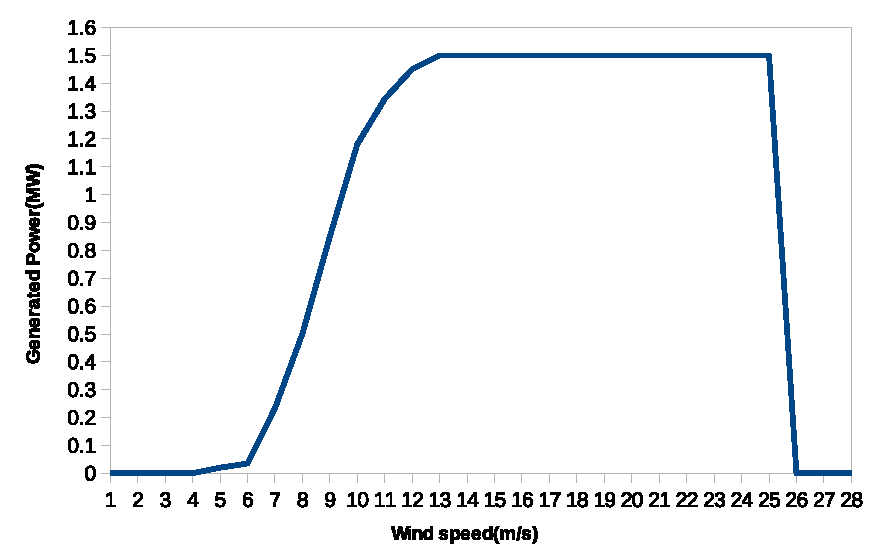
\includegraphics[width=1\columnwidth]{img/wind_curve.pdf}
\caption{Power curve of the GE 1.5MW wind turbine}
\label{fig:windcurve}
\end{figure}
%%%


\begin{table}[ht]
\begin{center}
\caption{Wind farm settings}
\begin{tabular}{|l|l|c|c|}
\hline
WF No. & Bus No. & State & Capacity(MW) \\
\hline
WF1 & 18& New Hampshire & 100\\
WF2 & 28& Maine & 90 \\
WF3 & 36& Vermont & 90  \\
WF4 & 37& Maine & 90\\
WF5 & 38& Massachusetts & 90\\
\hline

\end{tabular}
   \vspace{.05in}
\label{tab:wf_setting}
\end{center}
\end{table}
}
\end{itemize}
\subsection{Case study}
We have used the above described model and carried out the following case studies to assess the impact of datacenter location on the renewable power grid.
\begin{itemize}
\item{Case 1: Existing New England system}
\item{Case 2: New England system with one additional datacenter (co-located with a wind farm)}
\item{Case 3: New England system with one additional datacenter (located away from the wind farm)}
\end{itemize}
For assessing the impact, we use the three metrics described earlier (section \ref{sec:intro}) and calculate the system losses, power flows through the transmission lines and the bus voltages.
The system losses, line flows and the bus voltages are calculated by solving the power flow or loadflow equations. The loadflow equations mathematically model the power balance (i.e., net load +losses = total generation in the electric grid). Within an electric grid the power can be easily measured at the loads and at generators. Also, some generators have the capability to regulate the voltage at a bus at a constant preset reference value. The power flow equations are used to calculate the bus voltages (magnitude and angle), for a given network and a set of load and generation powers. The loadflow equation for a generic $n$ bus network with $k$ branches is given below.
\begin{equation}
P_{i} = \Sigma_{j=1}^{n}(|Y_{ij}||V_{i}||V_{j}|cos(\theta_{ij}+\delta_{j}-\delta_{i})
\end{equation}
\begin{equation}
Q_{i} = -\Sigma_{j=1}^{n}(|Y_{ij}||V_{i}||V_{j}|sin(\theta_{ij}+\delta_{j}-\delta_{i})
\end{equation}
where $P_{i}$ and $Q_{i}$ are real and reactive powers at the $i^{th}$ bus; $|V_{i}| \angle \delta_{i}$ is the voltage magnitude and angle at the the $i^{th}$ bus; $|Y_{ij}| \angle \theta_{ij}$ is the admittance of the branch between $i^{th}$ and $j^{th}$ bus.
For a given power $P_{i}$ and $Q_{i}$ at the $i^{th}$ load bus, the above powerflow equations are used to solve for the voltage magnitude and angle at the $i^{th}$ bus. Since the above equations, i.e., real and reactive powers are non-linear function of voltage they are solved iteratively using Newton Raphson method. Once the bus voltages are calculated the line flows and system losses are computed.
\subsection{Results and discussion}
%I need only the following results for each case (Case1, Case2 and Case 3):
%1. a table containing system losses for each case (total loss its only one number for each case)
%2. any line capacity violations (line number)
%3. voltage violations if any (bus number)
%%%

Here, with respect to the three cases mentioned above, we calculate line power flows, bus voltages and the value of system losses respectively by conducting simulation experiments, and then discuss the results under the condition of different placement choices for the datacenter.

First, we perform the experiment using peak system load (6885MW in total) and gain an insight of the impact of datacenter placement on line overloading situations. Wind speed setting here is LOW (4-6m/s), which means the power generated by the wind farm is nearly zero (less than 2.3\% of the rated capacity). Evaluation results are illustrated in Table \ref{tab:results-linevio}, which shows that there is one overloaded branch from bus 4 to bus 5 in Case 2. This highlights that different placement choice of the additional datacenter can make some particular lines overloaded. During our experiments, although there are only a few cases where lines are overloaded, annually the number of times and how long these over-loads could occur depends on the frequency and duration of occurrence of a particular wind speed and load condition. If it is too frequent or more persistent then the over-loads could be a serious problem and might require building new transmission lines. According to \cite{interconnection2010survey}, the estimated cost of building new transmission lines of 345kV voltage level is about \$2.5 Million/mile, which is very expensive with total costs in the billions of dollars. Hence, it's important to choose the right place for datacenters in order to mitigate line over-loading occurrences.


\begin{table}[ht]
\begin{center}
\caption{Results of overloaded lines}
\begin{tabular}{|c|c|c|}
\hline
Case No. & \# of overloaded lines & List of overloaded lines \\
\hline
1 & 0 & None\\
2 & 1 &  bus 4 - bus 5 \\
3 & 0 & None \\

\hline

\end{tabular}
   \vspace{.05in}
\label{tab:results-linevio}
\end{center}
\end{table}

Then, we investigate cases illustrating voltage variation of the electric grid, as shown in Table \ref{tab:results-volvio}. Here, the wind speed setting is MEDIUM (8-10m/s), which means the generated power of the wind turbine will be 33.3\%-78.7\% of its rated capacity. For Case 2 the datacenter is located at bus 38 (co-located with wind farm 5), and for Case 3 the datacenter is located at bus 25 (away from wind farms). The acceptable voltage range of a bus is set to [0.95p.u.,1.05p.u.]. It can be observed under this condition, there is already voltage deviation happening on one bus of the original New England system. When we choose a place for the datacenter co-locating with a wind farm as Case 2, the number of buses with voltage deviation will increase to four. If we don't restrict to co-located datacenter placement, we can find other possible choices (e.g. Case 3) to eliminate the unacceptable voltage deviation from nominal values. This result highlights that by carefully choosing the place for the datacenter might mitigate large voltage variations of the electric grid.

\begin{table}[ht]
\begin{center}
\caption{Results of voltage variations}
\begin{tabular}{|c|p{1in}|p{1in}|}
\hline
Case No. & \# of buses with voltage deviation & List of buses with voltage deviation  \\
\hline
1 & 1 & bus25\\
\hline
2 & 4 & \tabincell{c}{bus25\\bus26\\bus28\\bus29}\\
\hline
3 & 0 & None \\

\hline

\end{tabular}
   \vspace{.05in}
\label{tab:results-volvio}
\end{center}
\end{table}

At last, the total system losses are compared over the three cases under the condition of three wind speed settings, as shown in Figure~\ref{fig:loss-cases}. Here, the background load of the electric grid is set to normal (6254MW in total,summarized over all the buses). Three categories of wind speed settings are: LOW, MEDIUM, and HIGH. The setting HIGH means the wind speed is larger than 11m/s, and the output power of the wind turbine is nearly reaching its rated capacity. For example, a 100MW wind farm is generating at least 89.6MW power under this setting. The size of the additional datacenter in Case 2\&3 is set to 200MW. Specifically, for Case 2 the datacenter is located at bus 18 (co-located with wind farm 1) and for Case 3 the datacenter is located at bus 10 (away from all wind farms).

\begin{figure}[ht]
\centering
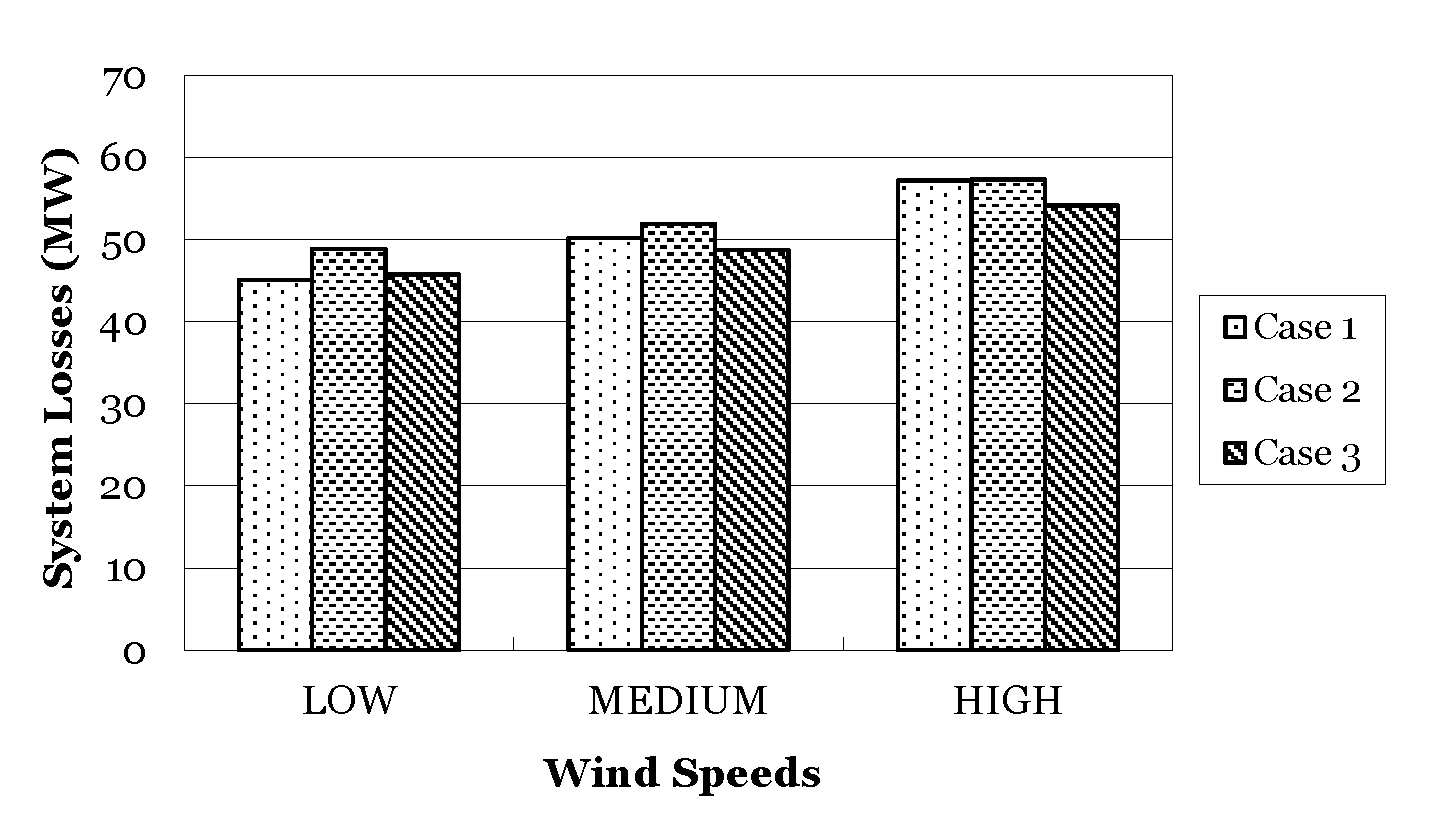
\includegraphics[width=1\columnwidth]{img/loss3cases.pdf}
\caption{Results of system losses}
\label{fig:loss-cases}
\end{figure}

By comparing the values of system losses from Figure~\ref{fig:loss-cases}, it can be observed that the co-location case (Case 2) could lead to more losses than Case 1 and Case 3. Take MEDIUM setting for example, the system losses of Case 3 is about 6\% less than Case 2, which illustrates system loss can be reduced by placing the datacenter correctly and co-location is not necessarily the best choice.


Note that even though we have provided one set of results for a particular set of condition, we have simulated different wind speed and load conditions. We found that in general the system loss magnitude could change. However, in most cases we saw that co-location is not the optimal choice for minimum system loss. In Section \ref{sec:framework} we will describe a method for determining the datacenter location that will correspond to minimal system loss annually and will cover all the wind speed and system load conditions.

